\documentclass[12pt]{scrartcl}

\usepackage{authblk}
\usepackage[natbib,authordate,backend=bibtex]{biblatex-chicago}
   \bibliography{references}
\usepackage{booktabs}
\usepackage{csquotes}
\usepackage{enumitem}
\usepackage{float}
\usepackage[top=4cm,bottom=4cm,left=3cm,right=2.5cm]{geometry}
\usepackage[hidelinks]{hyperref}
   \urlstyle{same}
\usepackage[utf8]{inputenc}
\usepackage{longtable}
\usepackage{siunitx}
\usepackage{tabto}
\usepackage{tikz}

\deffootnote{1.5em}{1em}{\makebox[1.5em][l]{\thefootnotemark}}
   \setlength{\skip\footins}{1.5em} 
   \setlength{\footnotesep}{1em}

\renewcommand\Affilfont{\small}

\NumTabs{14}

\title{Answers at Gunpoint}
\subtitle{On Livengood and Sytsma's Revolver Case}

\author[1]{Alexander Max Bauer}
\author[2]{Jan Romann}

\affil[1]{ Department of Philosophy, University of Oldenburg,

Corresponding Author, E-Mail: \href{mailto:alexander.max.bauer@uni-oldenburg.de}{alexander.max.bauer@uni-oldenburg.de}}
\affil[2]{ SOCIUM Research Center on Inequality and Social Policy, University of Bremen}

\date{\small 2023\\\textit{Philosophy of Science} 89 (1), 180--192}

\begin{document}
\maketitle

\begin{abstract}
   \noindent\textbf{\textsf{Abstract:}} Jonathan Livengood and Justin Sytsma have published a series of studies on \textit{Actual Causation and Compositionality}, in which they investigate causal attributions of laypeople. We use one of their vignettes to follow up on their research. Our findings cast doubt on their conclusion that ordinary causal attributions tend to violate the compositionality constraint if one looks at cases in which someone is responsible for an effect by way of an intermediary that does not share in the responsibility.
\end{abstract}

\section{Introduction}
\citet*{livengood_actual_2020} have published a series of studies on \textit{Actual Causation and Compositionality}. Theories of actual causation, they argue, often at least implicitly endorse a so-called \textit{compositionality constraint}: Imagine that someone, let's name him Alrik, set up a row of domino tiles. He gave the first tile a flick and as the result of a chain reaction, all the other tiles were knocked over, too. The first tile's falling over was \textit{directly} caused by Alrik's flick. Since subsequently all the other tiles tumbled over, too, Alrik's flick did also cause the last tile in the chain to fall. It was not directly but \textit{indirectly} caused by Alrik's flick. Here, the flick caused some intermediary tiles to fall, which in turn caused the last tile to fall. This can be expressed in a more abstract way: If we look at some individual events, henceforth denoted as \textit{c}, \textit{d}, and \textit{e}, the compositionality constraint states that if the event \textit{c} caused the event \textit{e}, then it did so either directly or it did so indirectly via one or more intermediaries \textit{d}. In this case, every intermediary \textit{d} is itself an effect of \textit{c} and a cause of \textit{e} \citep[44]{livengood_actual_2020}.

This compositionality constraint intuitively seems to be a reasonable desideratum for any adequate theory of actual causation. However, whether it is indeed correct, Livengood and Sytsma argue, is a different kettle of fish. Arguably, it is not enough to solely rely on the intuitions of a single philosopher or of a small, relatively homogeneous group of thinkers.\footnote{Also see \citet*{bauer_two_2020}.} Here, the \textit{folk attribution desideratum} \citep{livengood_following_2017} comes into play. This condition of adequacy demands \enquote{that what a theory of actual causation says about concrete, everyday cases [has to] accord with ordinary causal attributions} \citep[48]{livengood_actual_2020}. This in mind, \citeauthor*{livengood_actual_2020} set out to find answers regarding the question whether or not causal attributions of laypeople comply with the compositionality constraint. Previous research has already shown that laypeople's causal attributions are influenced by normative judgements about what someone ought to do. In light of this, \citet*[48]{livengood_actual_2020} formulate their main hypothesis:
%
\begin{quote}
   \small [O]rdinary causal attributions will tend to violate the compositionality constraint for cases in which someone or something is responsible for an effect by way of an intermediary that does not share in the responsibility.
\end{quote}
%
To test this hypothesis, they set up a number of vignette studies, each introducing a short story that contains information on certain agents, their intentions, as well as a causal sequence of events, containing some intermediaries. Subsequent to each vignette, they asked participants to rate their agreement or disagreement with certain statements about causation in the given story. Their first vignette \citep[49]{livengood_actual_2020}, e.\,g., states:
%
\begin{quote}
   \small Amy wants to kill her daughter, Jessica, but she doesn't want to go to prison for murder. As such, Amy hatches a plan. She arranges for a baby sitter, Courtney, to take care of Jessica while she is out of town on business. Before leaving, Amy laces one of Jessica's sippy cups with a deadly poison that is very difficult to detect. That evening, Courtney gives Jessica juice in the poisoned sippy cup. Jessica drinks the juice and dies two hours later.
\end{quote}
%
Subsequent to reading this story, subjects were asked to rate their level of agreement or disagreement with the two statements \enquote{Amy caused Jessica's death} and \enquote{Courtney caused Jessica's death} on a seven-point scale from 1 (\enquote{strongly disagree}) to 7 (\enquote{strongly agree}).

If the causal attributions of laypeople comply with the compositionality constraint, one would expect subjects to agree that intermediaries – in this case Courtney -- also cause the effect in question. Surprisingly, though, subjects tended to rate statements about the causal impact of intermediaries as rather low: For the example above, the responses suggested that the compositionality constraint was clearly violated, since subjects by and large agreed that Amy caused Jessica's death, but most of them denied that Courtney, too, caused Jessica's death. Similar results were obtained in the other studies Livengood and Sytsma report on. They found that most causal attributions by laypeople seem to violate the compositionality constraint across the vignettes they tested. Do these surprising results adequately depict laypeople's idea of actual causation? Or could it be the case that subjects had moral responsibility or blameworthiness in mind -- either unconsciously or consciously -- rather than the concept of actual causation? These findings, after all, might be in part the result of the way subjects were asked in the first place: Asking about the causal role of involved agents (either at the beginning or at the end of the causal chain) might have led subjects to misinterpret the questions in terms of responsibility. And the only (morally) accountable subject, in this case, would arguably be Amy. Of course, Livengood and Sytsma were well aware of this possibility, which is why they did not settle with those results but conducted a number of subsequent studies. In one of those studies, they introduced two human agents and a number of intermediaries that were mechanical instead of human. Yet, they obtained similar results. Again, it might be the case that subjects focused on the question of responsibility instead of causation. To give some first indications on this, we replicate this study with an altered set of questions to test the robustness of the original findings. In Section 2 of this discussion note, we will first introduce Livengood and Sytsma's study and findings briefly, before outlining our own study and findings in Section 3. Section 4 concludes the note.

\section{Livengood and Sytsma's Revolver Case}
Since this is a discussion note rather than a full-blown replication study, we focus on only one of the vignettes used by Livengood and Sytsma. Clearly, further research has to extend this focus. Here, we limit ourselves to their eighth case. It includes an agent (and thus someone being accountable), but in contrast to their previous studies, it presents a rather long chain of intermediaries that are not themselves human agents. This allows us to adopt the vignette while being able to easily alter the questions asked. Their vignette \citep[59]{livengood_actual_2020} reads:
%
\begin{quote}
   \small Trent has decided to kill his father, Brad. He aims his loaded revolver at Brad and pulls the trigger, releasing the hammer. The hammer strikes the cartridge, igniting the gun powder. The gun powder explodes, driving the bullet from the gun. The bullet hits Brad in the head. He dies instantly.
\end{quote}
%
Livengood and Sytsma asked 51 subjects to rate their level of agreement or disagreement on a seven-point scale from 1 (\enquote{strongly disagree}) to 7 (\enquote{strongly agree}) with four statements on causal attribution, namely: (1) \enquote{Trent caused Brad's death}, (2) \enquote{The hammer caused Brad's death}, (3) \enquote{The gun powder caused Brad's death}, and (4) \enquote{The bullet caused Brad's death}. Again, if laypeople's causal attributions comply with the compositionality constraint and subjects say that Trent caused Brad's death, then they should also state that the hammer, the gunpowder, and the bullet caused Brad's death as well.

As can be seen in \autoref{fig:plot}, which compares the results from Livengood and Sytsma's study to ours, a  majority of their subjects completely or strongly agreed with the first statement that Trent caused Brad's death. Here, the central tendency of the responses was statistically above 4. For the second and third statement, though, the central tendency of the responses was statistically below 4, indicating that subjects did not ascribe causation to the intermediaries in question. For the last statement answers were bimodal. Here, the central tendency was not statistically different from 4. Sytsma and Livengood conclude that their findings suggest that the compositionality constraint is violated.

\section{The Revolver Case Reconsidered}
To test whether or not there might be some first indications that subjects from Livengood and Sytsma's studies understood the questions in terms of responsibility instead of actual causation, we repeat the study introduced above. To do so, we use the same vignette as they did but alter the set of questions. It is striking that every statement in the original version -- i.\,e., \enquote{Trent caused Brad's death}, \enquote{The hammer caused Brad's death}, \enquote{The gun powder caused Brad's death}, and \enquote{The bullet caused Brad's death} -- only asks for the causal attribution regarding the outcome, Brad's death. In this case, we assume, the focus on Brad's death could easily lead subjects to misinterpret causation as responsibility. This might be less the case, we presume, when subjects are additionally asked about statements that refer not to Brad's death but to other steps of the causal chain that do not include human agents. We think that this could make the framing of actual causation more salient. To achieve this, we divide the vignette up into a number of events as follows:
%
\begin{itemize}
   \item\textbf{\textsf{Event A:}} \enquote{pulling the trigger}
   \item\textbf{\textsf{Event B:}} \enquote{releasing the hammer}
   \item\textbf{\textsf{Event C:}} \enquote{striking the cartridge}
   \item\textbf{\textsf{Event D:}} \enquote{igniting the gun powder}
   \item\textbf{\textsf{Event E:}} \enquote{the gun powder exploding}
   \item\textbf{\textsf{Event F:}} \enquote{driving the bullet from the gun}
   \item\textbf{\textsf{Event G:}} \enquote{the bullet hitting Brad in the head}
   \item\textbf{\textsf{Event H:}} \enquote{the death of Brad}
\end{itemize}
%
Next, we combine those events to statements of the form \enquote{X caused Y}, resulting in 28 different items that include all reasonable combinations of events to be made therefrom, e.\,g., \enquote{Pulling the trigger caused the release of the hammer}, \enquote{Striking the cartridge caused the ignition of the gun powder}, or \enquote{The bullet being driven from the gun caused the bullet to hit Brad in the head} (see \autoref{app:combinations} for a full list of items).

As in the original study by Livengood and Sytsma, subjects were asked to state their level of agreement or disagreement with each of those 28 items on a seven-point scale from 1 (\enquote{strongly disagree}) to 7 (\enquote{strongly agree}). If the results of Livengood and Sytsma are robust, we should get similar responses not only for their first item but also for their second, third, and fourth item when comparing them to a similar event in our causal chain. Due to our method of constructing the statements, the formulations are slightly different in our study; nonetheless, we consider the following items to be analogous:
%
\begin{itemize}
   \item The first statement from Livengood and Sytsma, \enquote{Trent caused Brad's death}, is similar to our item \enquote{Pulling the trigger caused the death of Brad} (A/H in \autoref{app:combinations}).
   \item The second statement, \enquote{The hammer caused Brad's death}, is similar to our item \enquote{Releasing the hammer caused the death of Brad} (B/H in \autoref{app:combinations}).
   \item The third statement, \enquote{The gun powder caused Brad's death}, is similar to our items \enquote{Igniting the gun powder caused the death of Brad} and \enquote{The explosion of the gun powder caused the death of Brad} (D/H and E/H in \autoref{app:combinations}).
   \item The fourth statement, \enquote{The bullet caused Brad's death}, is similar to our items \enquote{The bullet being driven from the gun caused the death of Brad} and \enquote{The bullet hitting Brad in the head caused the death of Brad} (F/H and G/H in \autoref{app:combinations}).\footnote{One might notice that in doing so, we assume that people make judgements about agents or objects on the one hand and actions or events on the other hand in analogous ways. While this is something research has to explore more deeply in the future, we can, for now, note that \citet*{livengood_following_2017} did not find differences when emphasising actions as opposed to agents, similar to \citet*{livengood_actual_2020} when emphasising objects as opposed to agents.}
\end{itemize}
%
Our study was programmed in \cite{limesurvey_project_team_limesurvey_2020} and was conducted online in April 2020. Subjects were students from the University of Oldenburg, recruited with the help of the Graduate School for Social Sciences and Humanities. A book voucher worth 20 euros was raffled off between all participants. No approval was sought from the ethics commission since this is a survey using hypothetical vignettes and assessing uncritical opinions. Altogether there were 52 non-native English speakers, of whom 22 identified as female, three as diverse, and 26 as male (one missing value). The mean age was 27.58 (median: 25), with two participants not indicating their age.\footnote{Data can be retrieved from \url{https://github.com/alephmembeth/causality-revolver}.}

On the first page, subjects were greeted with a welcome screen (see \autoref{app:welcome}). Subsequently, they were shown the vignette together with instructions and the first set of items (see \autoref{app:vignette} and \ref{app:screens}). Items were presented in an ordered sequence, split into seven groups (as depicted in \autoref{app:combinations}, see also \autoref{app:screens}) that were presented on separate screens.

\begin{figure}[th!]
   \centering
   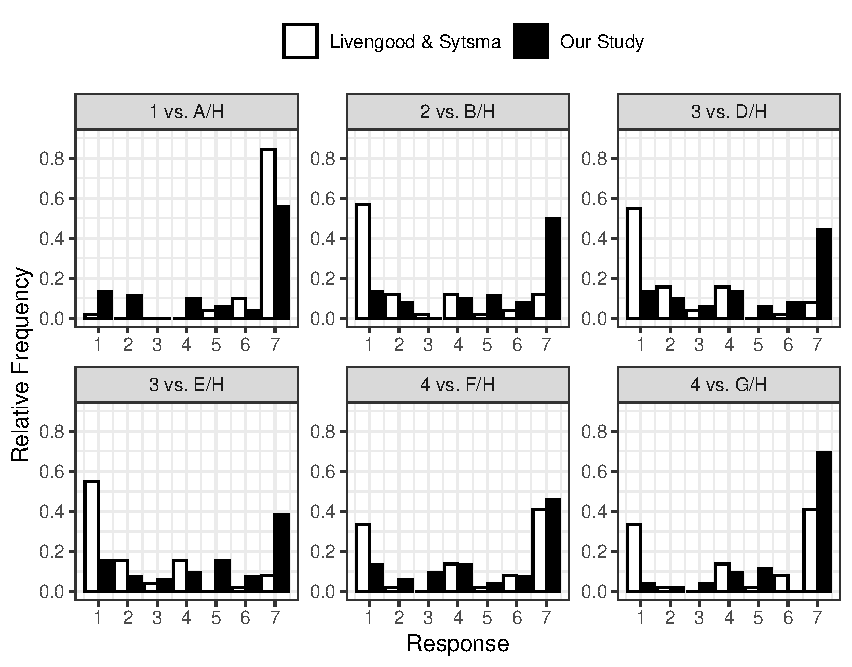
\includegraphics[width=\textwidth]{figures/comparison.pdf}
   \begin{minipage}{\linewidth}
      \emph{Note: White bars represent the data from Livengood and Sytsma (1 = \enquote{Trent caused Brad's death}, 2 = \enquote{The hammer caused Brad's death}, 3 = \enquote{The gun powder caused Brad's death}, 4 = \enquote{The bullet caused Brad's death}), black bars represent our data (A/H = \enquote{Pulling the trigger caused the death of Brad}, B/H = \enquote{Releasing the hammer caused the death of Brad}, D/H = \enquote{Igniting the gun powder caused the death of Brad}, E/H = \enquote{The explosion of the gun powder caused the death of Brad}, F/H = \enquote{The bullet being driven from the gun caused the death of Brad}, G/H = \enquote{The bullet hitting Brad in the head caused the death of Brad}). We assume that cases 1 and A/H, 2 and B/H, 3 and D/H, 3 and E/H, 4 and F/H, as well as 4 and G/H are analogous.}
   \end{minipage}
   \caption{Bar charts for the cases from Livengood and Sytsma vs. our analogous cases.}
   \label{fig:plot}
\end{figure}

\noindent\autoref{fig:plot} displays the evaluations for the cases identified as analogues to those presented by Livengood and Sytsma. Our first statement is evaluated similarly to the one presented by them. The majority of our subjects strongly agrees that \enquote{Pulling the trigger caused the death of Brad}. Here, the central tendency of the responses is significantly above 4 (A/H: $V = 876.5, p < 0.001, \Delta = 0.404$ [$0.145,$ $0.611$]).\footnote{We use Wilcoxon matched-pairs signed-rank tests to reject the hypothesis that the central tendency for each statement is less than or equal to the \enquote{neutral} value of 4, as did Livengood and Sytsma. The \emph{R} package \emph{effsize}, authored by \cite{torchiano_effsize_2020}, was used to calculate Cliff's delta for our comparisons.} There is a striking difference between our results and those from Livengood and Sytsma, though, when we turn to the second statement. Here, the majority of our subjects continues to strongly agree that \enquote{Releasing the hammer caused the death of Brad} (B/H: $V = 869, p < 0.001, \Delta= 0.481 \left[0.228, 0.673\right]$). The same holds true for the statements \enquote{Igniting the gun powder caused the death of Brad} (D/H: $V = 756, p = 0.01, \Delta = 0.289 \left[0.032, 0.509\right]$), \enquote{The explosion of the gun powder caused the death of Brad} (E/H: $V = 780, p = 0.02, \Delta = 0.327 \left[0.065, 0.547\right]$), \enquote{The bullet being driven from the gun caused the death of Brad} (F/H: $V = 772, p < 0.001$, $\Delta = 0.288 \left[0.032, 0.509\right]$), and \enquote{The bullet hitting Brad in the head caused the death of Brad} (G/H: $V = 1053, p < 0.001, \Delta = 0.712 [0.495, 0.845]$). This is in stark contrast to the results of Livengood and Sytsma. Where their subjects did not attribute causation or the picture was not clear, our subjects continued to ascribe causation.

Not only for the cases above but for every single item of ours an (oftentimes overwhelming) majority of subjects chose to \enquote{strongly agree} that \enquote{X caused Y}. Moreover, Wilcoxon matched-pairs signed-rank tests reject the hypothesis that the central tendency for any of the 28 combinations is smaller than or equal to the \enquote{neutral} answer 4 (see \autoref{tab:summary} and \autoref{tab:wilcoxon} in \autoref{app:tables} for summary statistics and test results).

\section{Conclusion}
Our findings allow for the conjecture that it might indeed be a confusion of actual causation and responsibility that lies behind the surprising findings of Livengood and Sytsma. Instead of showing what subjects think about actual causation, their data might more or less show what their subjects think about responsibility. In this case, their results would not adequately depict laypeople's idea of actual causation. This might be the case, we suspect, because they oftentimes prominently feature human agents, as we have seen with the two studies presented above: First, the vignettes introduced human agents alongside their morally questionable intentions (\enquote{Amy wants to kill her daughter} or \enquote{Trent has decided to kill his father}). Second, subjects were asked to indicate their agreement with statements focusing on the causation of a morally undesired outcome (e.\,g., \enquote{Courtney caused Jessica's death} or \enquote{The hammer caused Brad's death}). Taken together, this might have triggered a desire to blame.\footnote{The assumption of blame as a driving factor behind causal judgements is well established in the literature \citep[see, e.\,g.,][]{alicke_culpable_2010,alicke_causation_2011,alicke_culpable_2012,danks_demoralizing_2014,rose_folk_2017,sytsma_causation_2020}.} If this is the driving force, then our design might have had a de-biasing effect, making considerations of causation more salient than considerations of responsibility. While Livengood and Sytsma only asked about the causal relation between very few domino tiles, so to speak, we asked subjects to evaluate the broader picture. Presenting a large number of statements that mostly refer to mechanical actions rather than human agents and that additionally point out all the possible causal relations they have, might have led subjects to actually have causation in mind rather than responsibility, since they were forced to reflect on a number of causal relations that clearly had nothing to do with responsibility. This might have shifted the focus away from the blameworthy agent and reduced the effect of subjects' desire to blame.\footnote{This could also be understood loosely as a framing effect: The same vignette and the analogue items are perceived differently given the context of the other items.}

This in mind, our findings cast doubt on the conclusion of Livengood and Sytsma that odinary causal attributions tend to violate the compositionality constraint if we look at cases in which someone is responsible for an effect by way of an intermediary that does not share in the responsibility. Said cases, we assume from our data, fail to make a convincing case against the constraint, as long as the differences between our results and those from Livengood and Sytsma are not explained sufficiently. This opens up a number of questions: Might our results be generalizable in that people always or mostly conform to the compositionality constraint but recent studies failed to make the question of causality salient? This could have widespread consequences. Should our results turn out to be robust they might suggest that there is -- at least in this regard -- no gap between theoretical constructs and folk ideas of actual causation after all. \citet[64f.]{livengood_actual_2020} state that \enquote{even philosophers, such as Lewis and Menzies, explicitly giving analyses of the ordinary concept of causation have offered theories that entail the compositionality constraint}, and then continue asking: \enquote{How could they have gotten things so wrong?} It turns out that they might not have been wrong after all. For now, it seems, they can uphold their theoretical assumptions.

Of course, we only tested one of the many studies from Livengood and Sytsma. Since they mainly varied the vignettes and not the way they asked their subjects, we suspect that similar effects would occur. This needs further testing, though, which is beyond the scope of this discussion note.

Moreover, there is a vast number of possible follow-up questions: Does a close proximity of events (say, A/B, B/C, C/D, \dots) entail a higher rating of causation compared to other combinations of events? Or does human agency have such an effect (as in A/B, A/C, A/D, \dots, see also \cite{rose_folk_2017})? And how do evaluations differ when -- as was the case for most studies by Livengood and Sytsma -- we look at interpersonal relations (as in A/H)?

Lastly, it has to be noted that the ontological category of the causal relata could make a difference. Livengood and Sytsma asked for the \textit{objects} (\enquote{the hammer}, \enquote{the gun powder}, and \enquote{the bullet}), we asked for the related \textit{events} (i.\,e., \enquote{releasing the hammer} or \enquote{igniting the gun powder}). As noted above, \citet*{livengood_following_2017} did not find differences when emphasising actions as opposed to agents, similar to \citet*{livengood_actual_2020} when emphasising objects as opposed to agents. Whether or not our different findings are also influenced by this ontological difference needs to be addressed in further studies.

As can be seen from these questions, there is much to be done.

\section*{Acknowledgements}
First and foremost, we thank Jonathan Livengood and Justin Sytsma for interesting impulses and exciting exchanges, as well as for sharing their data and \textit{R} files with us. Malte Ingo Meyerhuber, Stephan Kornmesser, and Mark Siebel provided insightful comments. Rea Kodalle kindly helped to find participants for our study. Ewgenia Baraboj carefully proofread this discussion note. We are indebted to them all. We also thank four anonymous reviewers who provided helpful comments to this discussion note.

\clearpage
\appendix
\section{Items}
\label{app:combinations}
\subsection*{Group A}
\noindent\textbf{\textsf{A/B:}}\tab Pulling the trigger caused the release of the hammer.\\
\noindent\textbf{\textsf{A/C:}}\tab Pulling the trigger caused the hammer to strike the cartridge.\\
\noindent\textbf{\textsf{A/D:}}\tab Pulling the trigger caused the ignition of the gun powder.\\
\noindent\textbf{\textsf{A/E:}}\tab Pulling the trigger caused the explosion of the gun powder.\\
\noindent\textbf{\textsf{A/F:}}\tab Pulling the trigger caused the bullet to be driven from the gun.\\
\noindent\textbf{\textsf{A/G:}}\tab Pulling the trigger caused the bullet to hit Brad in the head.\\
\noindent\textbf{\textsf{A/H:}}\tab Pulling the trigger caused the death of Brad.

\subsection*{Group B}
\noindent\textbf{\textsf{B/C:}}\tab Releasing the hammer caused the hammer to strike the cartridge.\\
\noindent\textbf{\textsf{B/D:}}\tab Releasing the hammer caused the ignition of the gun powder.\\
\noindent\textbf{\textsf{B/E:}}\tab Releasing the hammer caused the explosion of the gun powder.\\
\noindent\textbf{\textsf{B/F:}}\tab Releasing the hammer caused the bullet to be driven from the gun.\\
\noindent\textbf{\textsf{B/G:}}\tab Releasing the hammer caused the bullet to hit Brad in the head.\\
\noindent\textbf{\textsf{B/H:}}\tab Releasing the hammer caused the death of Brad.

\subsection*{Group C}
\noindent\textbf{\textsf{C/D:}}\tab Striking the cartridge caused the ignition of the gun powder.\\
\noindent\textbf{\textsf{C/E:}}\tab Striking the cartridge caused the explosion of the gun powder.\\
\noindent\textbf{\textsf{C/F:}}\tab Striking the cartridge caused the bullet to be driven from the gun.\\
\noindent\textbf{\textsf{C/G:}}\tab Striking the cartridge caused the bullet to hit Brad in the head.\\
\noindent\textbf{\textsf{C/H:}}\tab Striking the cartridge caused the death of Brad.

\subsection*{Group D}
\noindent\textbf{\textsf{D/E:}}\tab Igniting the gun powder caused the explosion of the gun powder.\\
\noindent\textbf{\textsf{D/F:}}\tab Igniting the gun powder caused the bullet to be driven from the gun.\\
\noindent\textbf{\textsf{D/G:}}\tab Igniting the gun powder caused the bullet to hit Brad in the head.\\
\noindent\textbf{\textsf{D/H:}}\tab Igniting the gun powder caused the death of Brad.

\subsection*{Group E}
\noindent\textbf{\textsf{E/F:}}\tab The explosion of the gun powder caused the bullet to be driven from the gun.\\
\noindent\textbf{\textsf{E/G:}}\tab The explosion of the gun powder caused the bullet to hit Brad in the head.\\
\noindent\textbf{\textsf{E/H:}}\tab The explosion of the gun powder caused the death of Brad.

\subsection*{Group F}
\noindent\textbf{\textsf{F/G:}}\tab The bullet being driven from the gun caused the bullet to hit Brad in the head.\\
\noindent\textbf{\textsf{F/H:}}\tab The bullet being driven from the gun caused the death of Brad.

\subsection*{Group G}
\noindent\textbf{\textsf{G/H:}}\tab The bullet hitting Brad in the head caused the death of Brad.

\section{Welcome Message}
\label{app:welcome}
Welcome to this short survey. You won't need more than fifteen minutes to complete it.

Among all participants who answer this survey by Saturday, April 19, an Amazon voucher worth 20 euros will be raffled off.

On the following pages, we will present you with a scenario and ask you to assess your agreement or disagreement with different statements that are made about this scenario.

Please read both the scenario's description and the task carefully.

Thank you for participating!

\section{Vignette and Instructions}
\label{app:vignette}
Trent has decided to kill his father, Brad. He aims his loaded revolver at Brad and pulls the trigger, releasing the hammer. The hammer strikes the cartridge, igniting the gun powder. The gun powder explodes, driving the bullet from the gun. The bullet hits Brad in the head. He dies instantly.

Please rate your level of agreement or disagreement with the following statements below. 1 represents \enquote{strongly disagree}, 4 is \enquote{neutral}, and 7 represents \enquote{strongly agree}.

\section{Example Screens}
\label{app:screens}
\begin{figure}[H]
   \centering
   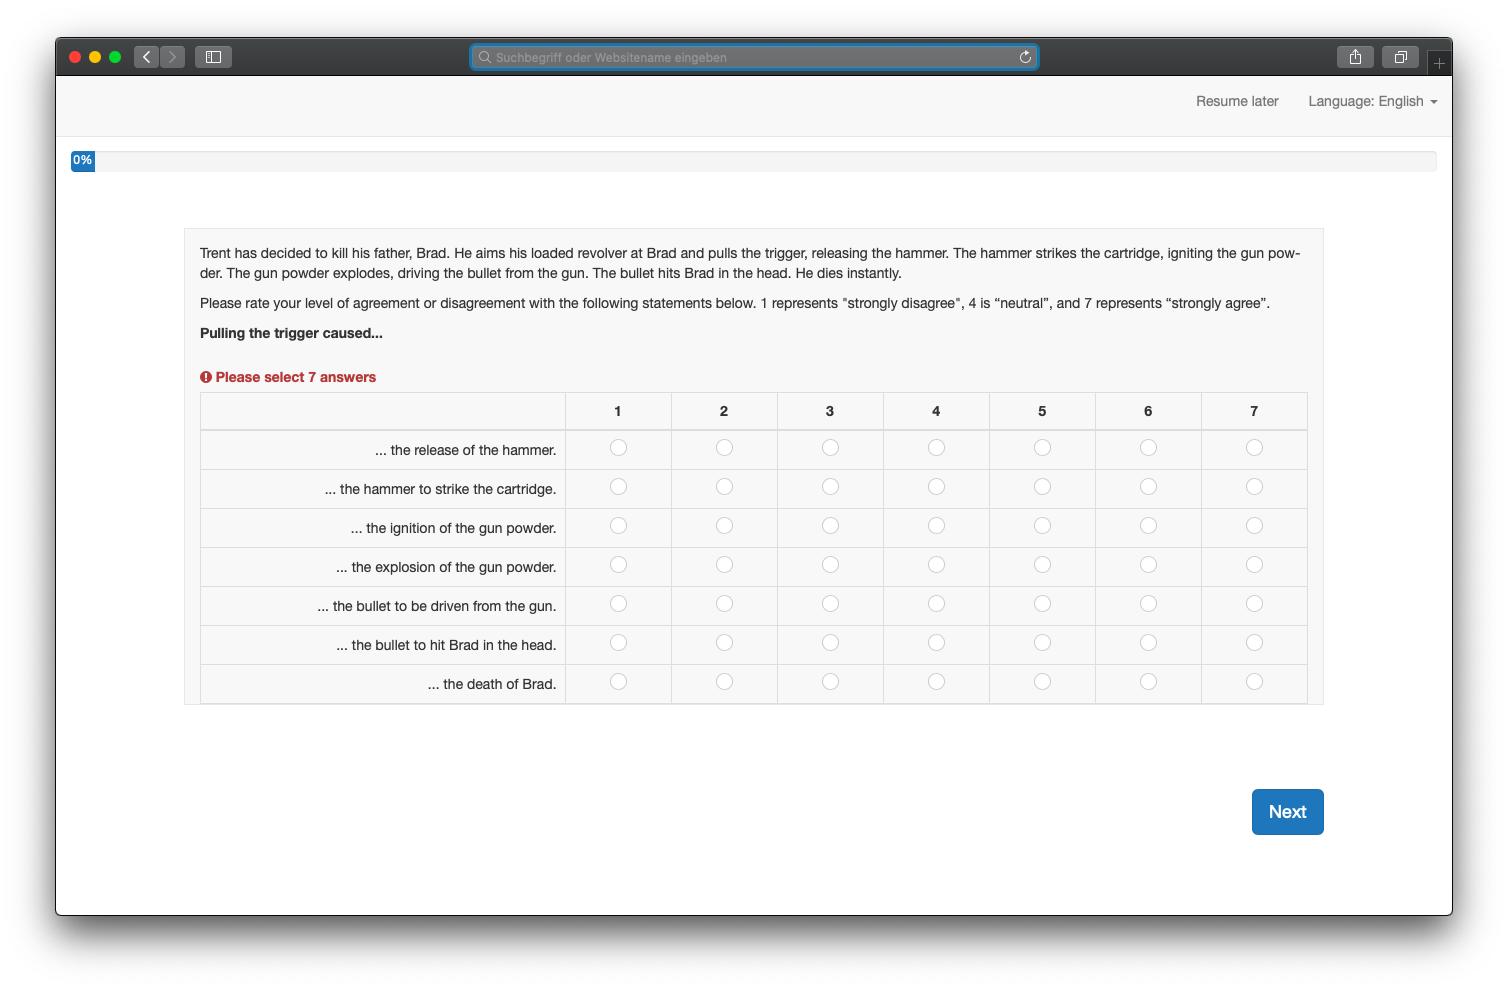
\includegraphics[width=0.85\textwidth]{figures/screen_1.png}
   \caption{Example of the first screen with questions shown to subjects.}
   \label{fig:screen_1}
\end{figure}

\begin{figure}[H]
   \centering
   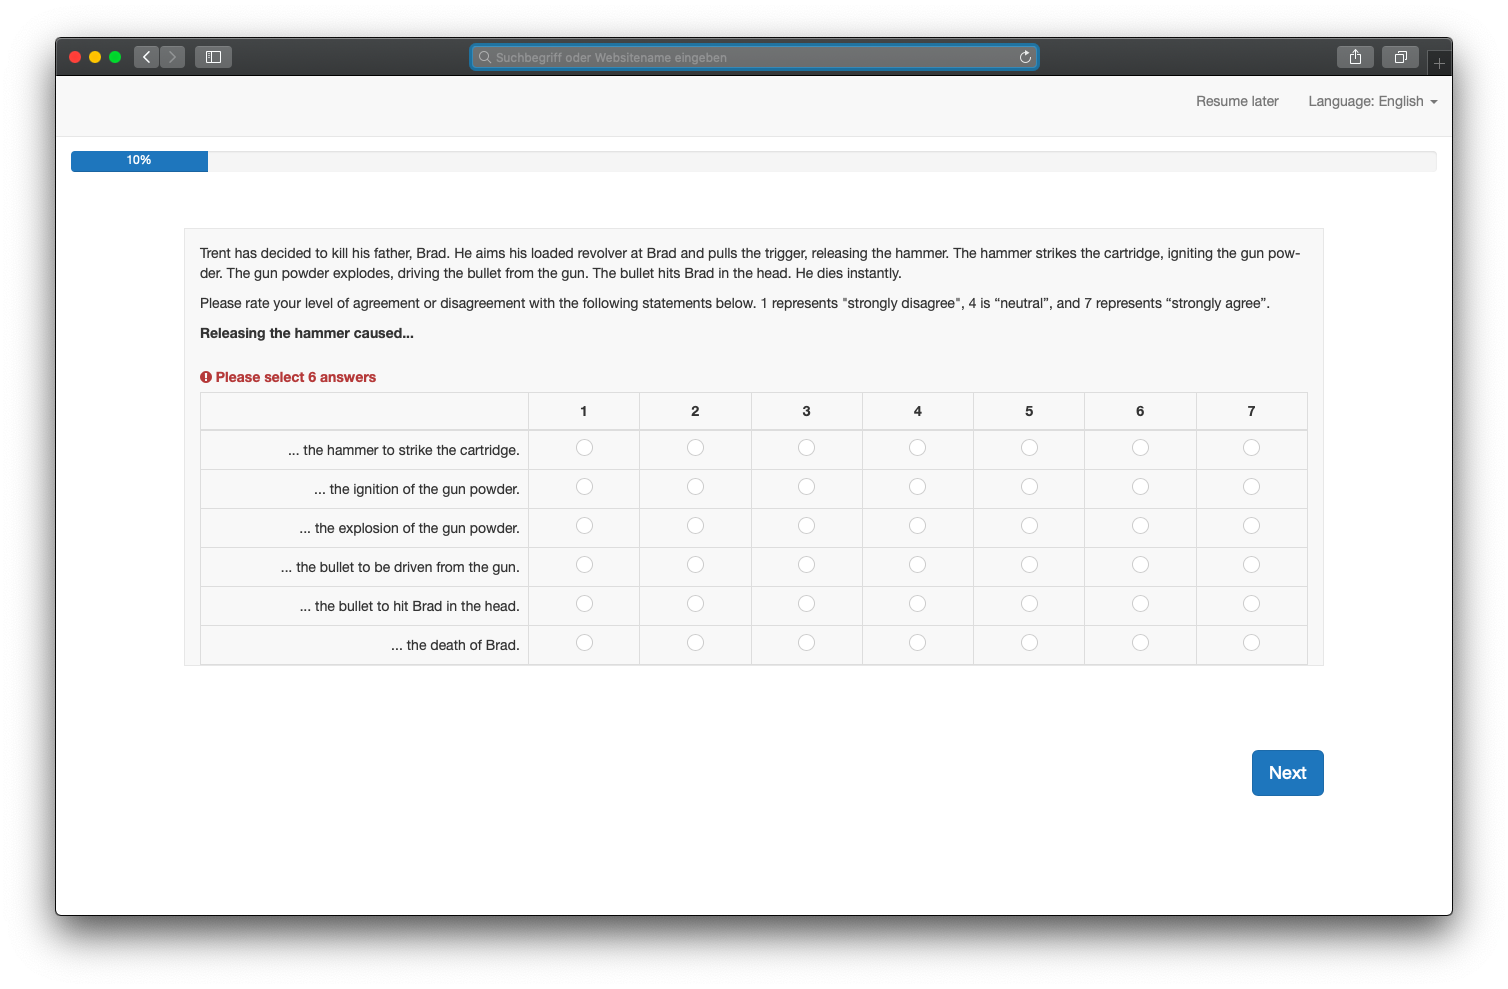
\includegraphics[width=0.85\textwidth]{figures/screen_2.png}
   \caption{Example of the second screen with questions shown to subjects.}
   \label{fig:screen_2}
\end{figure}

\clearpage
\section{Tables}
\label{app:tables}
\begin{longtable}{lSScS}
   \caption{Summary table for all statements.}
   \label{tab:summary}\\
   \toprule
   \multicolumn{1}{c}{Statement} & \multicolumn{1}{c}{Mean} & \multicolumn{1}{c}{Standard Error} & \multicolumn{1}{c}{95\% Confidence Interval} & \multicolumn{1}{c}{Variance}\\
   \midrule
   \endfirsthead
   \multicolumn{5}{c}{Table \thetable: Summary table for all statements (continued).}\\
   \toprule
   \multicolumn{1}{c}{Statement} & \multicolumn{1}{c}{Mean} & \multicolumn{1}{c}{Standard Error} & \multicolumn{1}{c}{95\% Confidence Interval} & \multicolumn{1}{c}{Variance} \\
   \midrule
   \endhead
   \multicolumn{5}{r}{{\emph{Continued on next page}}}\\
   \bottomrule
   \endfoot
   \bottomrule
   \endlastfoot
   A/B   & 5.89   & 0.26   & [5.37, 6.40]   & 3.48   \\*
   A/C   & 5.56   & 0.27   & [5.02, 6.10]   & 3.74   \\*
   A/D   & 5.33   & 0.28   & [4.77, 5.88]   & 4.00   \\*
   A/E   & 5.12   & 0.29   & [4.54, 5.70]   & 4.34   \\*
   A/F   & 5.19   & 0.28   & [4.63, 5.75]   & 4.08   \\*
   A/G   & 4.92   & 0.31   & [4.31, 5.54]   & 4.86   \\*
   A/H   & 5.17   & 0.33   & [4.51, 5.83]   & 5.64   \\
   \midrule
   B/C   & 5.90   & 0.27   & [5.37, 6.44]   & 3.70   \\*
   B/D   & 5.67   & 0.25   & [5.17, 6.18]   & 3.28   \\*
   B/E   & 5.25   & 0.27   & [4.71, 5.79]   & 3.80   \\*
   B/F   & 5.17   & 0.28   & [4.62, 5.73]   & 4.00   \\*
   B/G   & 4.90   & 0.30   & [4.31, 5.50]   & 4.56   \\*
   B/H   & 5.21   & 0.31   & [4.59, 5.84]   & 5.07   \\
   \midrule
   C/D   & 5.75   & 0.28   & [5.18, 6.32]   & 4.19   \\*
   C/E   & 5.54   & 0.26   & [5.02, 6.05]   & 3.43   \\*
   C/F   & 5.21   & 0.28   & [4.65, 5.77]   & 4.01   \\*
   C/G   & 4.69   & 0.32   & [4.06, 5.32]   & 5.16   \\*
   C/H   & 4.94   & 0.32   & [4.29, 5.59]   & 5.47   \\
   \midrule
   D/E   & 5.94   & 0.27   & [5.41, 6.48]   & 3.70   \\*
   D/F   & 5.58   & 0.25   & [5.07, 6.08]   & 3.27   \\*
   D/G   & 4.94   & 0.30   & [4.35, 5.53]   & 4.53   \\*
   D/H   & 4.88   & 0.32   & [4.24, 5.53]   & 5.32   \\
   \midrule
   E/F   & 5.92   & 0.26   & [5.41, 6.44]   & 3.41   \\*
   E/G   & 4.88   & 0.30   & [4.28, 5.49]   & 4.70   \\*
   E/H   & 4.79   & 0.31   & [4.16, 5.42]   & 5.15   \\
   \midrule
   F/G   & 5.19   & 0.30   & [4.59, 5.79]   & 4.63   \\*
   F/H   & 4.96   & 0.32   & [4.33, 5.60]   & 5.21   \\
   \midrule
   G/H   & 6.00   & 0.24   & [5.53, 6.47]   & 2.86   \\
\end{longtable}

\def\sym#1{\ifmmode^{#1}\else\(^{#1}\)\fi}

\begin{center}
   \begin{longtable}{crc}
      \caption{Two-tailed Wilcoxon signed-rank tests for all statements. $p$-values were corrected using the false discovery rate method by \cite{benjamini_controlling_1995}.}
      \label{tab:wilcoxon}\\
      \toprule
      Case & \multicolumn{1}{c}{$V$} & Adjusted $p$-value\\
      \midrule
      \endfirsthead
      \multicolumn{3}{p{0.45\textwidth}}{Table \thetable: Two-tailed Wilcoxon signed-rank tests for all statements (continued).}\\
      \toprule
      Case & \multicolumn{1}{c}{$V$} & Adjusted $p$-value\\
      \midrule
      \endhead
      \multicolumn{3}{c}{\footnotesize \sym{*} $p<0.05$, \sym{**} $p<0.01$, \sym{***} $p<0.001$}\\
      \midrule
      \multicolumn{3}{r}{{\emph{Continued on next page}}}\\
      \bottomrule
      \endfoot
      \midrule
      \multicolumn{3}{c}{\footnotesize \sym{*} $p<0.05$, \sym{**} $p<0.01$, \sym{***} $p<0.001$}\\
      \bottomrule
      \endlastfoot
      A/B   & 1079.00   & $< 0.001$\sym{***}                       \\*
      A/C   & 1058.50   & $< 0.001$\sym{***}                       \\*
      A/D   &  998.00   & $< 0.001$\sym{***}                       \\*
      A/E   &  842.00   & $\phantom{< }0.001$\sym{**\phantom{*}}   \\*
      A/F   &  792.00   & $< 0.001$\sym{***}                       \\*
      A/G   &  872.00   & $\phantom{< }0.004$\sym{**\phantom{*}}   \\*
      A/H   &  876.50   & $< 0.001$\sym{***}                       \\
      \midrule
      B/C   & 1067.50   & $< 0.001$\sym{***}                       \\*
      B/D   &  978.50   & $< 0.001$\sym{***}                       \\*
      B/E   &  915.50   & $< 0.001$\sym{***}                       \\*
      B/F   &  794.00   & $< 0.001$\sym{***}                       \\*
      B/G   &  806.50   & $\phantom{< }0.004$\sym{**\phantom{*}}   \\*
      B/H   &  869.00   & $\phantom{< }0.001$\sym{**\phantom{*}}   \\
      \midrule
      C/D   & 1152.50   & $< 0.001$\sym{***}                       \\*
      C/E   &  880.00   & $< 0.001$\sym{***}                       \\*
      C/F   &  891.50   & $< 0.001$\sym{***}                       \\*
      C/G   &  699.00   & $\phantom{< }0.035$\sym{*\phantom{**}}   \\*
      C/H   &  697.50   & $\phantom{< }0.005$\sym{**\phantom{*}}   \\
      \midrule
      D/E   & 1134.00   & $< 0.001$\sym{***}                       \\*
      D/F   &  986.00   & $< 0.001$\sym{***}                       \\*
      D/G   &  905.00   & $\phantom{< }0.004$\sym{**\phantom{*}}   \\*
      D/H   &  756.00   & $\phantom{< }0.006$\sym{**\phantom{*}}   \\
      \midrule
      E/F   & 1108.00   & $< 0.001$\sym{***}                       \\*
      E/G   &  722.50   & $\phantom{< }0.007$\sym{**\phantom{*}}   \\*
      E/H   &  780.00   & $\phantom{< }0.02$\sym{*\phantom{**}}    \\
      \midrule
      F/G   &  849.00   & $< 0.001$\sym{***}                       \\*
      F/H   &  772.00   & $\phantom{< }0.004$\sym{**\phantom{*}}   \\
      \midrule
      G/H   & 1053.00   & $< 0.001$\sym{***}                       \\
   \end{longtable}
\end{center}

\clearpage
\printbibliography

\end{document}
